\section{Zielsetzung}

Versuchsziel ist es, sich mit der Funktionsweise des Lock-In-Verstärkers vertraut zu machen. Außerdem soll für 10 verschiedene Phasen mit und ohne verrauschtes Signal die Funktionsweise verifiziert werden. Zuletzt soll die Rauschunterdrückung mit einer Photodetektorschaltung überprüft werden.

\section{Theorie}
\label{sec:Theorie}

Lock-In-Verstärker werden eingesetzt, um Signale mit hohem Rauschen zu messen. 
Im Gegensatz zum Bandpass kann hier auch Rauschen herausgefiltert werden, welches auf der selben Frequenz wie das Messsignal liegt.

Das zu messende Eingangssignal $U_\mathup{sig}$ durchläuft im Gerät verschiedene Bauelemente, die in Abbildung \ref{fig:lockin} dargestellt sind.
\begin{figure}
	\centering
		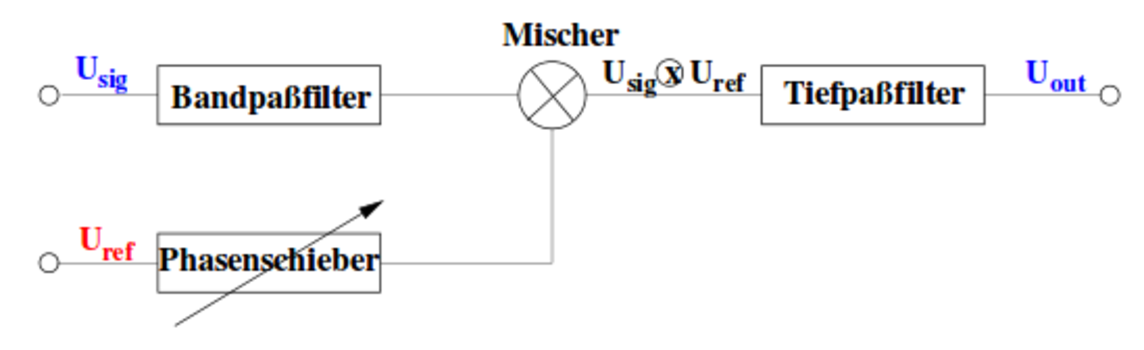
\includegraphics[width=\textwidth]{Bilder/LOCK_IN.pdf}
		\caption{Schematischer Aufbau des Lock-In-Verstärkers.}
		\label{fig:lockin}
	\end{figure}

Nach der Verstärkung durch den Pre-Amplifier durchläuft das Signal zunächst einen Bandpassfilter, der das Rauschen minimiert. 
Alle Frequenzen $\omega<<\omega_0$ und $\omega>>\omega_0$ werden grob herausgefiltert.
Ein Detektor erzeugt die Referenzspannung $U_\mathup{ref}$ -- eine Sinus- oder Rechteckspannung -- der Frequenz $\omega_0$, welche über den Phasenschieber an die Phase des Eingangssignals angepasst werden kann. 
Dieser Vorgang nennt sich Synchronisation.
Im Mischer treffen beide Signale aufeinander und werden multipliziert. Anschließend wird das Mischsignal $U_\mathup{sig}\times U_\mathup{ref}$ an den Tiefpass weitergeleitet, der die Modulationsfrequenz $\omega_0$ über mehrere Perioden integriert um restliche Rauschanteile $\omega\neq\omega_0$ auszuschließen. Zurück bleiben nur die Anteile der Signalsspannung $U_\mathup{sig}$, die mit der Referenzspannung synchronisiert werden konnten.

Um eine möglichst geringe Bandbreite $\Delta{\nu}=\frac{1}{\pi RC}$ zu erhalten, sollte die Zeitkonstante $\uptau=RC$ des Tiefpasses ausreichend groß gewählt werden. Damit wird eine hohe Güteziffer erzielt.

Die Ausgangsspannung $U_\mathup{out}$ ist eine Gleichspannung, welche proportional zur Eingangsspannung $U_\mathup{sig}$ und zum Cosinus der Phase ist: $U_\mathup{out}\propto{U_0}cos\Phi$. Je größer die Phasendifferenz zwischen Signal- und Referenzspannung ist, desto geringer ist die Ausgangsspannung. $U_\mathup{out}$ wird also maximal, wenn die Phasendifferenz $\Delta\Phi=0$ beträgt.
%Quellenangabe http://www.physik.uni-regensburg.de/studium/praktika/a2/download/versuch5a.pdf

\begin{figure}
	\centering
		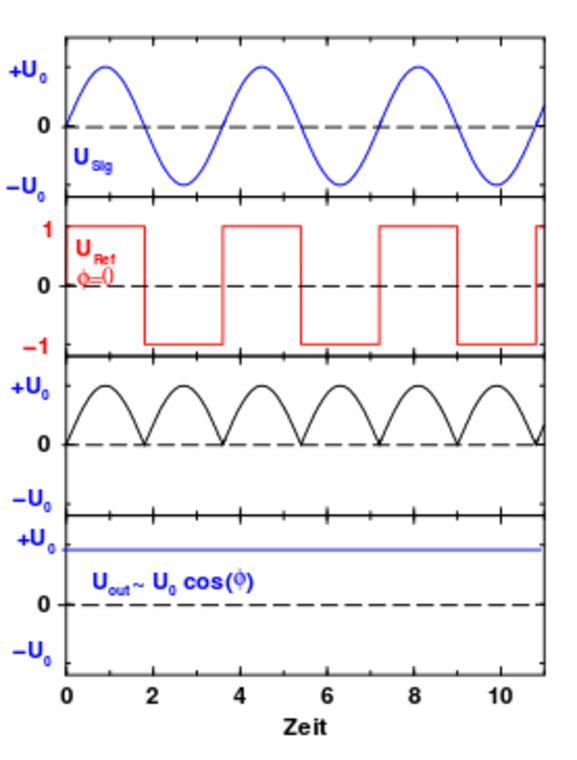
\includegraphics[width=0.5\textwidth]{Bilder/Beispiel.pdf}
		\caption{Überlagerung eines sinusförmigen Eingangssignals mit rechteckiger Referenzsspannung.}
		\label{fig:bsp}
	\end{figure}
Wird beispielsweise ein sinusförmiges Eingangssignal $U_\mathup{sig}=U_0sin(\omega t)$ wie in Abbildug \ref{fig:bsp} mit einem rechteckigen Referenzsignal $U_\mathup{ref}$ gleicher Frequenz überlagert, wird diese zunächst durch eine Fourierreihe angenähert, welche aus den ungeraden Harmonischen der Grundfrequenz besteht. Wird das multiplizierte Signal,  bestehend aus geraden Oberwellen der Frequenz $\omega$ durch den als Gleichrichter funktionierenden Tiefpass geleitet ergibt sich die Gleichspannung
\begin{equation}
U_\mathup{out}=\frac{2}{\pi}U_0cos(\Phi).
\end{equation}
Besteht kein Phasenunterschied zwischen Eingangs- und Referenzsignal nimmt die Ausgangsspannung ihren Maximalwert 
\begin{equation}
U_\mathup{out}=\frac{2}{\pi}U_0
\end{equation}
an.
Die Rechteckspannung mit auf 1 genormter Amplitude realisiert einen Schalter (\enquote{Chopper}). Indem die Werte 1 und -1 durch positive und negative Halbwellen angenommen werden, steht der Schalter auf \enquote{Ein} bzw. \enquote{Aus}.



